\documentclass{article}
\usepackage{graphicx}

\title{Answers}
\author{Timm Ruland \& Boris Prochnau}

\begin{document}
\maketitle

\begin{itemize}
\section{Task: 1}	%///////////////////////////////////
	\item What does it do? \\
it prints two not sufficiently seeded "random" variables
	\item The difference between the methods is that rand() returns a random number 
and the other method
  
	\begin{itemize}
		\item rand() returns a random integer between 0 and RANDMAX
		\item gsl\_rng\_mt19937 is a generator that generates random numbers
	\end{itemize}
 In the code the generator is passed to a (Distribution)function that uses this generator 
 to evaluate a random number depending on the Distribution specified in the function.
	\item What happens if you remove the expression (double)?\\
 The division operation $\frac{rand()}{RANDMAX}$ does $\frac{int Small}{int Big}$ and
 should result in a double, but with no cast it will be floored to 0. 
	\item Is there a direct function to generate normally distributed random variables?\\
	double gsl\_ran\_gaussian\_pdf(const gsl\_rng * r, double sigma)
 command
\end{itemize}

\newpage
\section{Task: 3} %//////////////////////////////////
The Plot should simulate the occurencedensity of points of our 1.000.000 samples which are normally distributed. But the picture
shows that all points are over the exact Plot of the density function what ist nearly impossible with so many samples. Therefor 
we conclude that the plot was made with different parameters.
\begin{figure}[h]
	\centering
		\includegraphics[width=0.70\textwidth]{E:/task3plot.eps}
	\label{fig:task3plot}
\end{figure}

\section{Task: 4} %//////////////////////////////////
We can sample a uniformlly y in the intervall [0,1] and apply the inverse cdf to sample a normally distributed variable

\newpage
\section{Task: 5} %//////////////////////////////////
The Algorithm uses a interpolation (see fig. 1) with maximal estimation error: $2*10^{-9}$ (see fig. 2) where the upper half of the Distributionfunction is devided into 2 sections in which interpolations where made. 
If x is in the lower halft of the Distributionfunction, than 1-NomralCDF(-x) will be used to use the symmetric property.
\begin{figure}[htbp]
	\centering
		\includegraphics[width=0.60\textwidth]{E:/pics/task5_interpolation_plot.eps}
		\caption{Plot of Approximation}
	\label{fig:task5_interpolation_plot}
\end{figure}
\begin{figure}[htbp]
	\centering
		\includegraphics[width=0.60\textwidth]{E:/pics/task5_difference_plot.eps}
	\caption{estimation error}
	\label{fig:task5_difference_plot}
\end{figure}

\newpage
\section{Task 6}
\begin{figure}[htbp]
	\centering
		
\includegraphics[width=0.50\textwidth]{E:/pics/task6_plot.eps}
	\caption{2D Plot}
	\label{fig:task6_plot}
\end{figure}

\section{Task 7}

\section{Task 8}
The algorithm need only one summation instead of two. The algorithm interates new samples to the total solution of the last step, so it could work better if we constantly give new sampels to the old ones because there is no need to run the hole calculation again. 

\section{Task 9}
We think that the error drops with the rate $\frac{1}{\sqrt{N}}$
\begin{figure}[htbp]
	\centering
		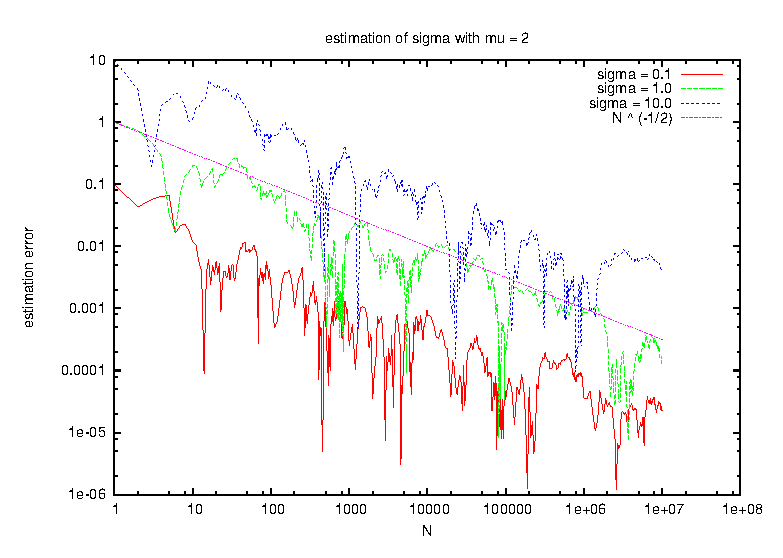
\includegraphics[width=0.50\textwidth]{E:/pics/task9_convergence_plot.eps}
	\caption{estimation error}
	\label{fig:task9_convergence_plot}
\end{figure}


\end{document}